\documentclass{article}
\bibliographystyle{livrevrel}
\usepackage{epubtk}
%\fi

\usepackage{graphicx}
\usepackage{amsmath}
\usepackage{amssymb}
\usepackage{textcomp}
\usepackage{xspace}
\usepackage{longtable}
\usepackage{multirow}

\newcommand{\mum}{\textmu\hspace{-0.2pt}m\xspace}
\newcommand{\muHz}{\textmu\hspace{-0.2pt}Hz\xspace}
\newcommand{\muN}{\textmu\hspace{-0.2pt}N\xspace}
\newcommand{\Hz}{Hz\super{-1/2}\xspace}
\newcommand{\HzHz}{Hz~Hz\super{-1/2}\xspace}

\begin{document}

\title{Gravitational Wave Detection by Interferometry (Ground and Space)
}

\author{%
\epubtkAuthorData{Matthew Pitkin}
        {Scottish Universities Physics Alliance (SUPA)\\
        School of Physics and Astronomy,\
        University of Glasgow \\
        Glasgow G12 8QQ, U.K.}
        {matthew.pitkin@glasgow.ac.uk}
        {}
\and
\epubtkAuthorData{Stuart Reid}
        {Scottish Universities Physics Alliance (SUPA)\\
        School of Physics and Astronomy,
        University of Glasgow \\
        Glasgow G12 8QQ, U.K.}
        {stuart.reid.2@glasgow.ac.uk}
    {}
\and
\epubtkAuthorData{Sheila Rowan}
        {Scottish Universities Physics Alliance (SUPA)\\
        School of Physics and Astronomy,
        University of Glasgow \\
        Glasgow G12 8QQ, U.K.}
        {sheila.rowan@glasgow.ac.uk}
        {}
\and
\epubtkAuthorData{Jim Hough}
        {Scottish Universities Physics Alliance (SUPA)\\
        School of Physics and Astronomy,
        University of Glasgow \\
        Glasgow G12 8QQ, U.K.}
        {james.hough@glasgow.ac.uk}
        {}
}

\date{}
\maketitle

\begin{abstract}\input{"./abstract"}\end{abstract}

\input{"./Section1"}

\begin{figure}[]
\begin{center}
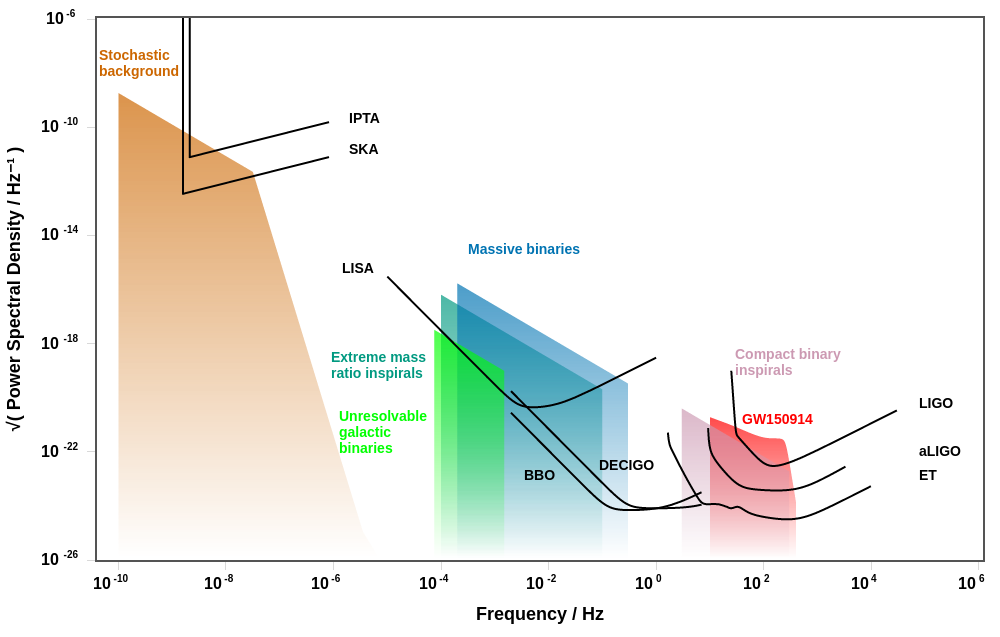
\includegraphics[width=1\columnwidth]{./figures/fig1/fig1}
\caption{ \protect\label{figure:sourcestrengths}
Some possible sources for ground-based and space-borne
    detectors.
}
\end{center}
\end{figure}

\input{"./Section2"}
\input{"./Section3"}

\begin{figure}[]
\begin{center}
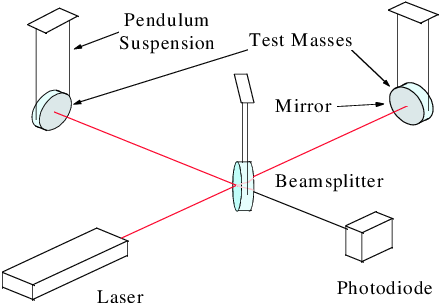
\includegraphics[width=1\columnwidth]{./figures/fig2/fig2}
\caption{ \protectSchematic of gravitational-wave detector using laser
    interferometry.}
\end{center}
\end{figure}


\begin{figure}[]
\begin{center}
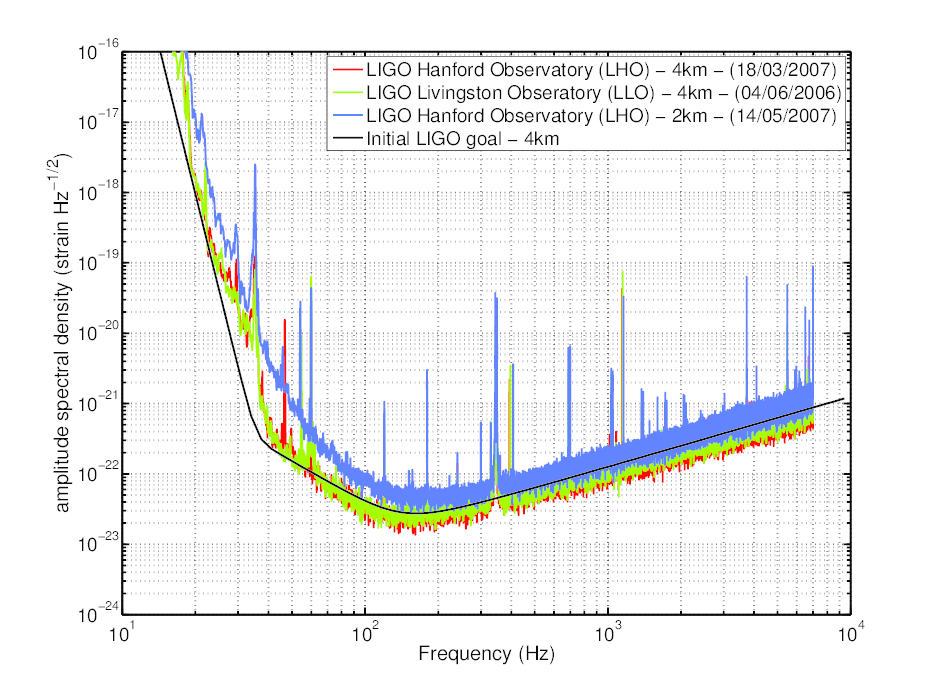
\includegraphics[width=1\columnwidth]{./figures/LIGOsens/LIGOsens}
\caption{ \protectMeasured sensitivity of the initial LIGO interferometers
    during the S5 science run (see
    Section~\ref{sec:ligoruns}). Reproduced with permission from
    \cite{LIGOcurves}.}
\end{center}
\end{figure}

\input{"./Section4"}

\begin{figure}[]
\begin{center}
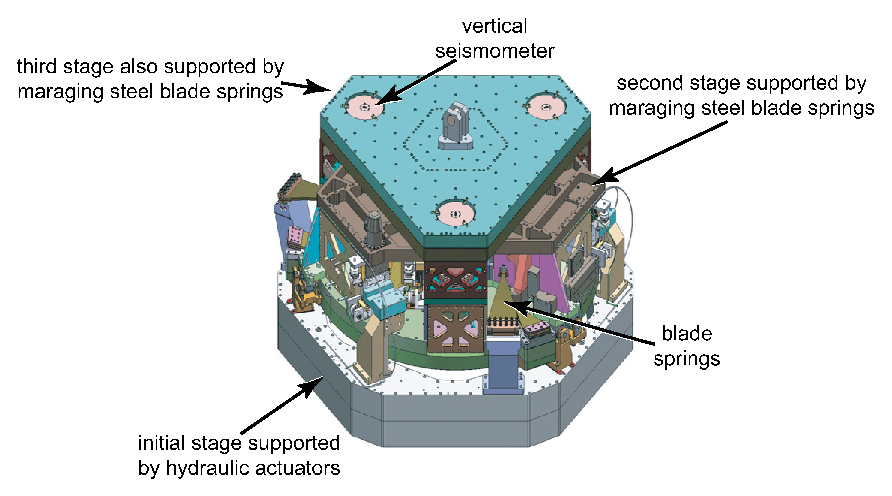
\includegraphics[width=1\columnwidth]{./figures/fig3/fig3}
\caption{ \protectInternal stages of the large chamber seismic isolation system
for Advanced LIGO (image is inverted for clarity).}
\end{center}
\end{figure}


\begin{figure}[]
\begin{center}
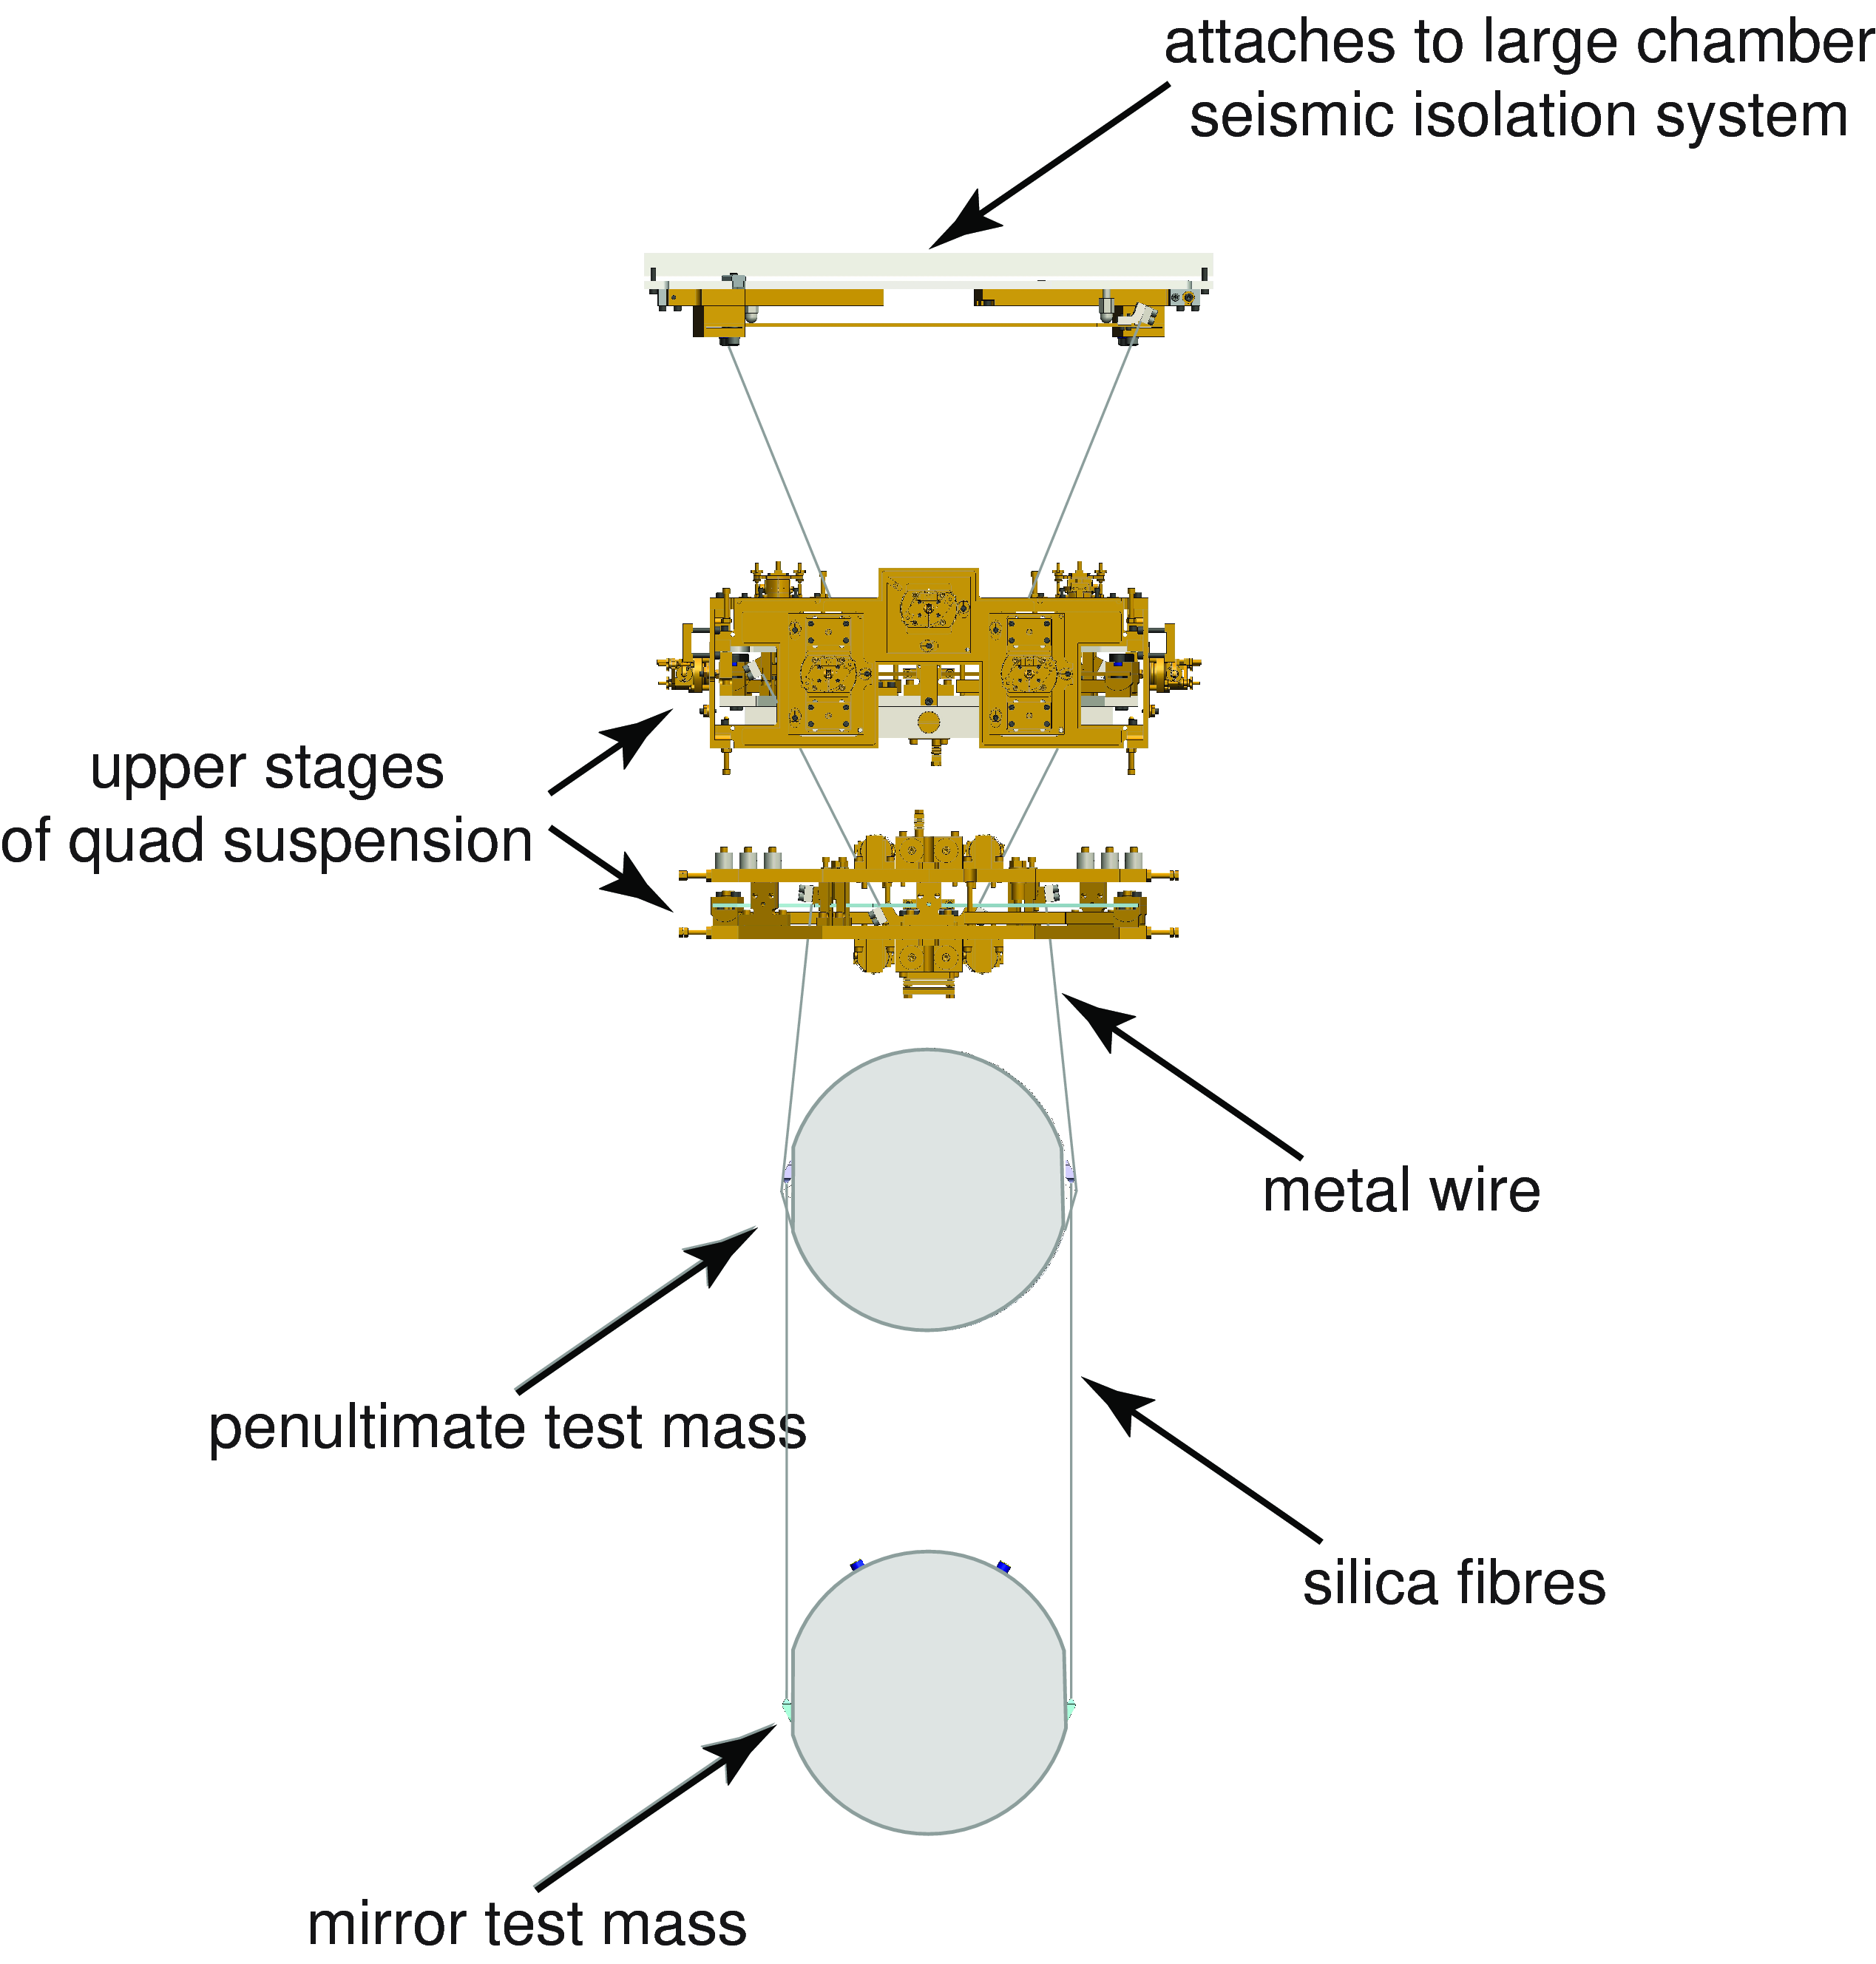
\includegraphics[width=1\columnwidth]{./figures/fig4/fig4}
\caption{ \protect\label{figure:LIGOquad}
CAD drawing of quad suspension system for Advanced LIGO, showing
the mirror test mass at the bottom and where the uppermost section is attached
to the third stage platform of the large chamber seismic isolation system shown
in Figure~\ref{figure:LIGOseismic}.
}
\end{center}
\end{figure}


\begin{figure}[]
\begin{center}
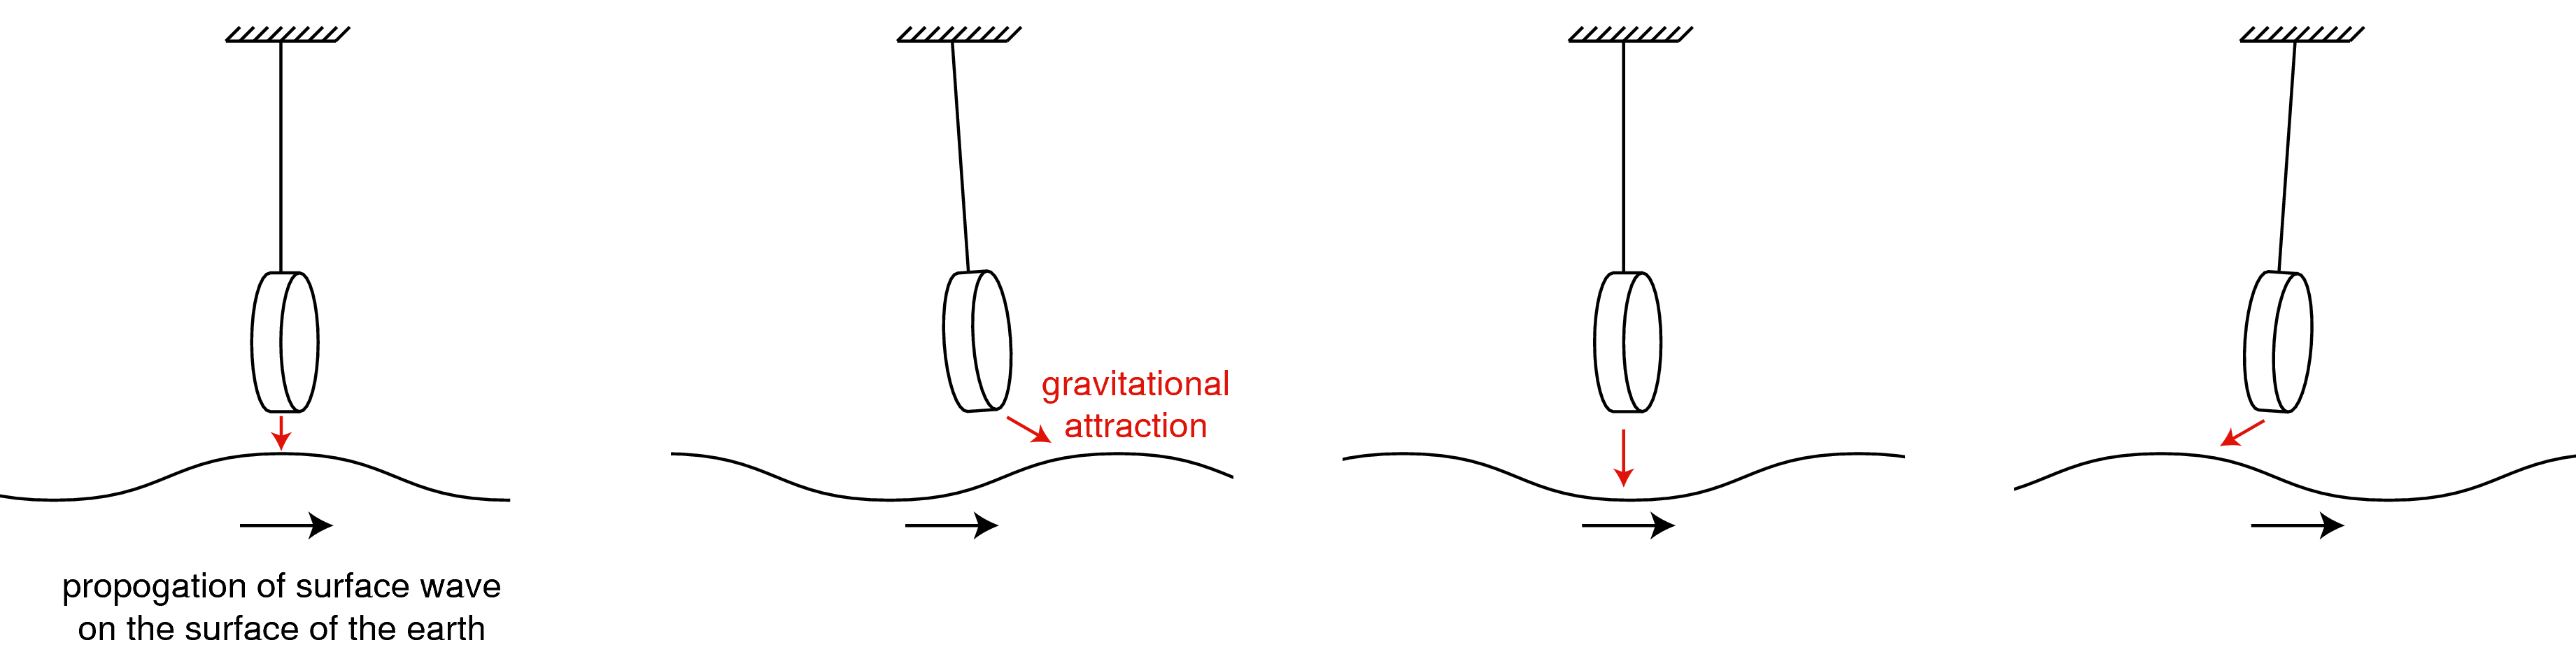
\includegraphics[width=1\columnwidth]{./figures/GGN/GGN}
\caption{ \protect\label{figure:GGN}
Time-lapsed schematic illustrating the fluctuating
    gravitational force on a suspended mass by the propagation of a
    surface wave through the ground.
}
\end{center}
\end{figure}


\begin{figure}[]
\begin{center}
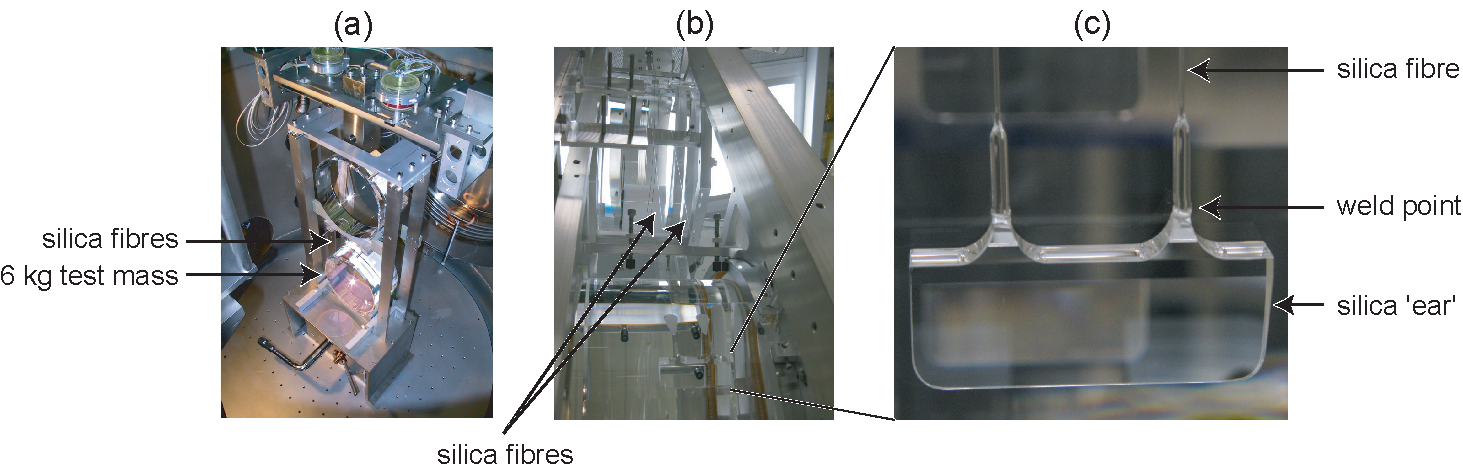
\includegraphics[width=1\columnwidth]{./figures/monolithic/monolithic}
\caption{ \protect\label{figure:monolithic}
Monolithic silica suspension of (a) GEO600 6~kg mirror test mass
suspended from 4 fibres of thickness 250~\mum and (b) prototype monolithic
suspension for Advanced LIGO at LASTI (mirror mass of 40~kg, silica fibre
thickness 400~\mum).
}
\end{center}
\end{figure}

\input{"./Section5"}

\begin{figure}[]
\begin{center}
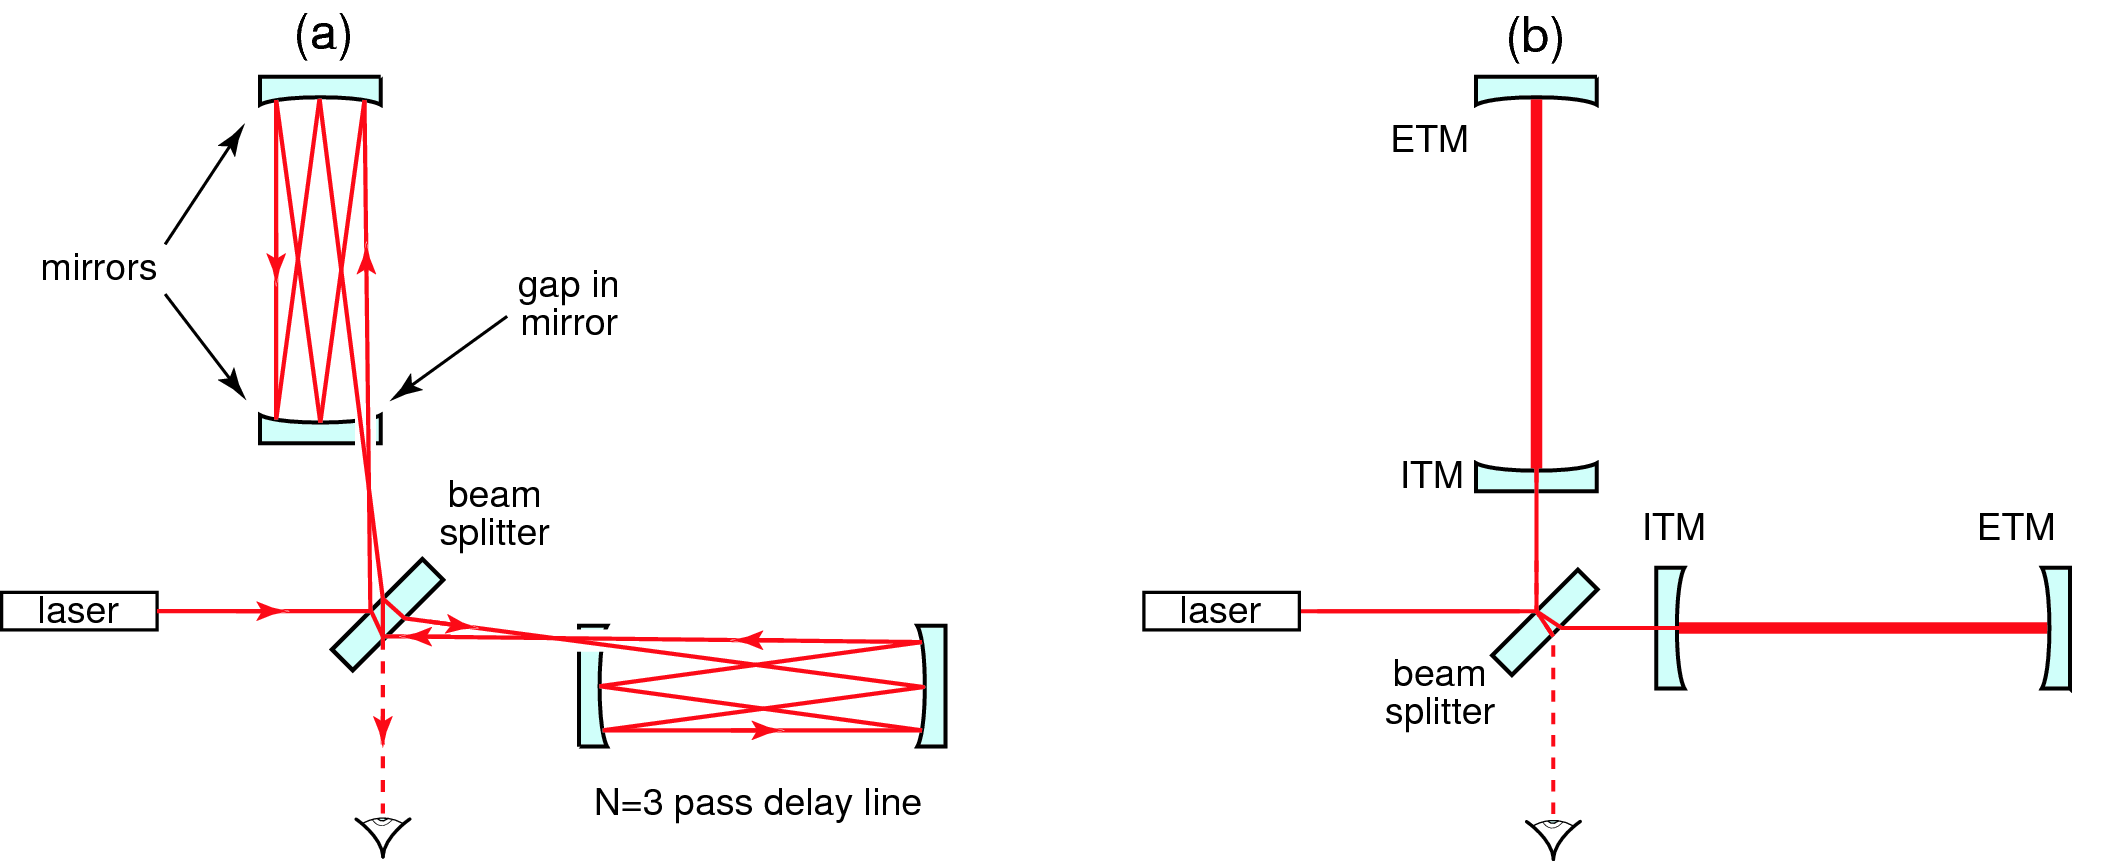
\includegraphics[width=1\columnwidth]{./figures/fig5e/fig5e}
\caption{ \protect\label{figure:Michelsons}
Michelson interferometers with (a) delay lines and (b)
Fabry--P\'{e}rot cavities in the arms of the interferometer.
}
\end{center}
\end{figure}


\begin{figure}[]
\begin{center}
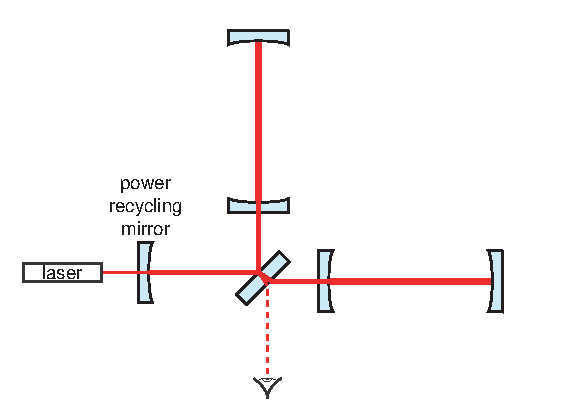
\includegraphics[width=1\columnwidth]{./figures/fig6a/fig6a}
\caption{ \protectThe implementation of power recycling on a
    Michelson interferometer with Fabry--P\'{e}rot cavities.}
\end{center}
\end{figure}


\begin{figure}[]
\begin{center}
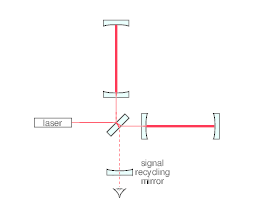
\includegraphics[width=1\columnwidth]{./figures/fig6b/fig6b}
\caption{ \protect\label{figure:Michelsons2b}
The implementation of signal recycling on a Michelson interferometer with Fabry--P\'{e}rot cavities.}
\end{center}
\end{figure}

\input{"./Section6"}

\begin{figure}[]
\begin{center}
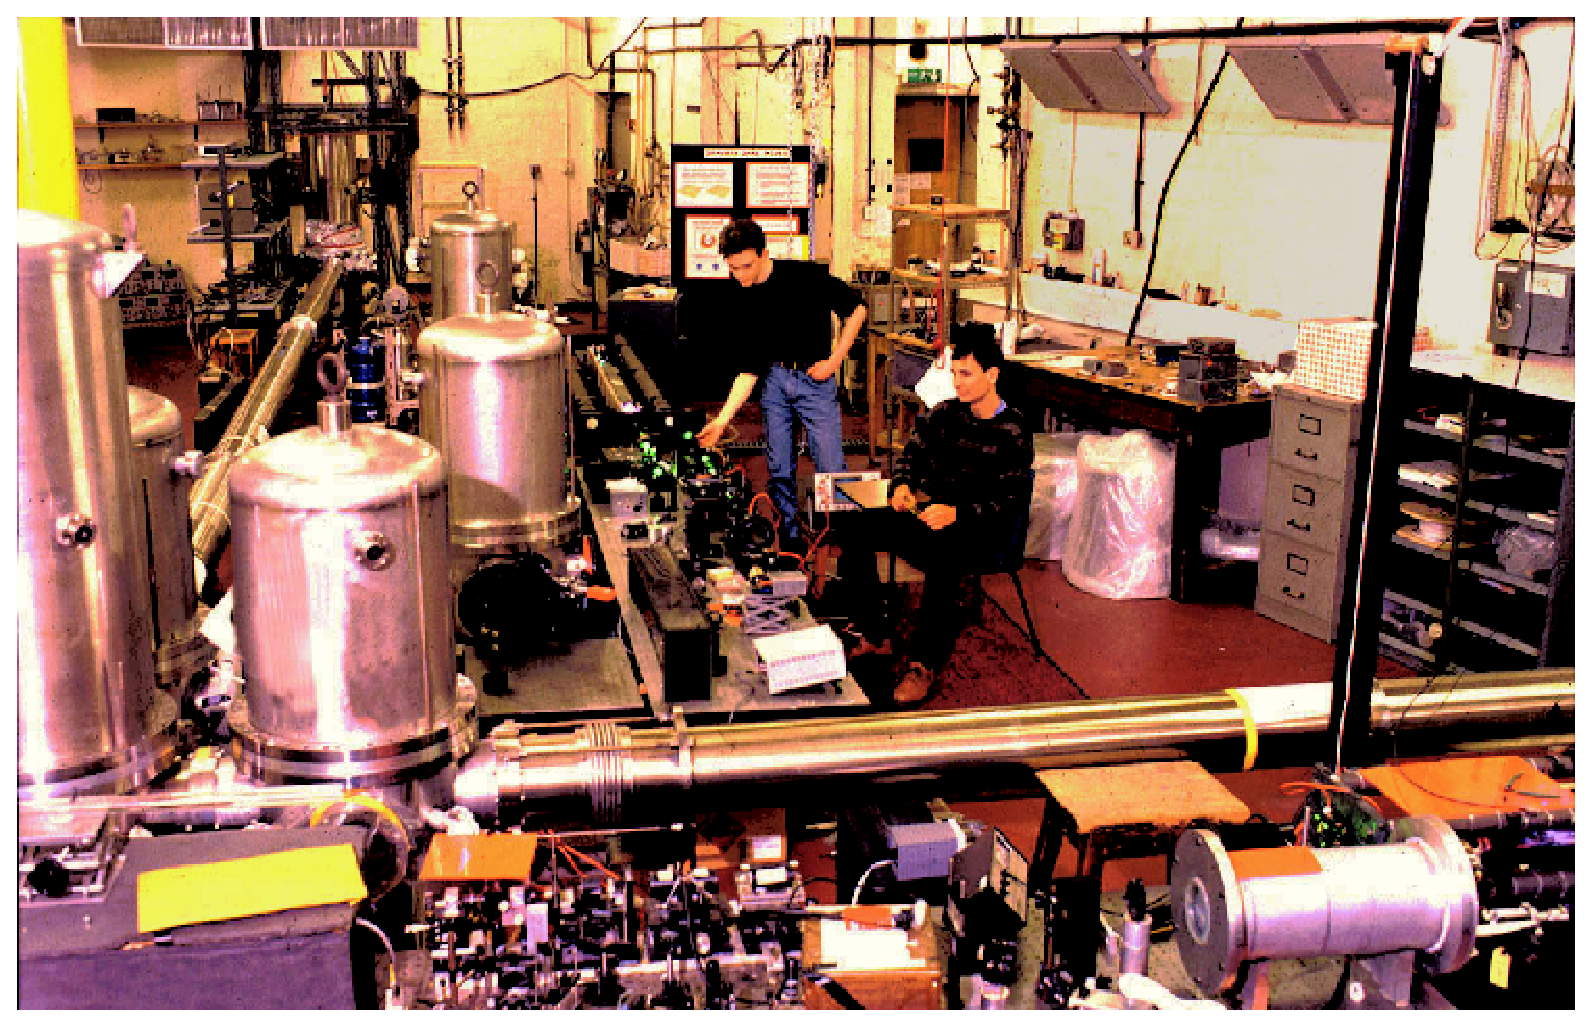
\includegraphics[width=1\columnwidth]{./figures/figpro/figpro}
\caption{ \protect\label{figure:Glasgowprototype}
The 10~m prototype gravitational wave detector
    at Glasgow.
}
\end{center}
\end{figure}


\begin{figure}[]
\begin{center}
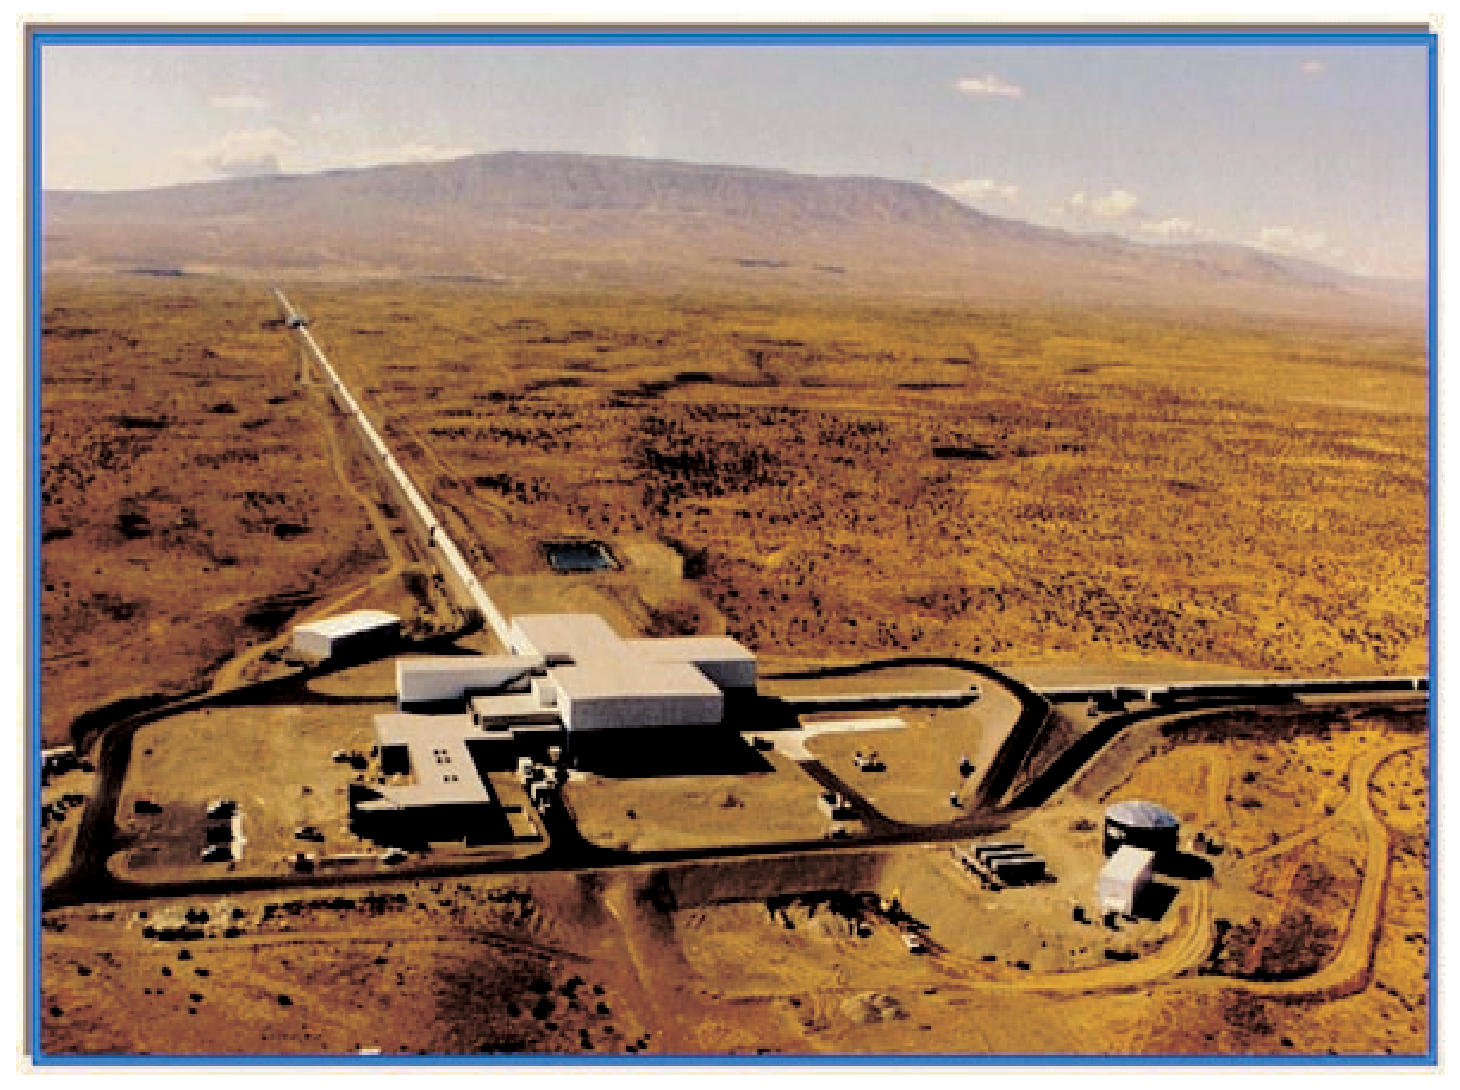
\includegraphics[width=1\columnwidth]{./figures/fig7/fig7}
\caption{ \protect\label{figure:LIGOsite}
A bird's eye view of the LIGO detector, sited in Hanford, Washington.}
\end{center}
\end{figure}


\begin{figure}[]
\begin{center}
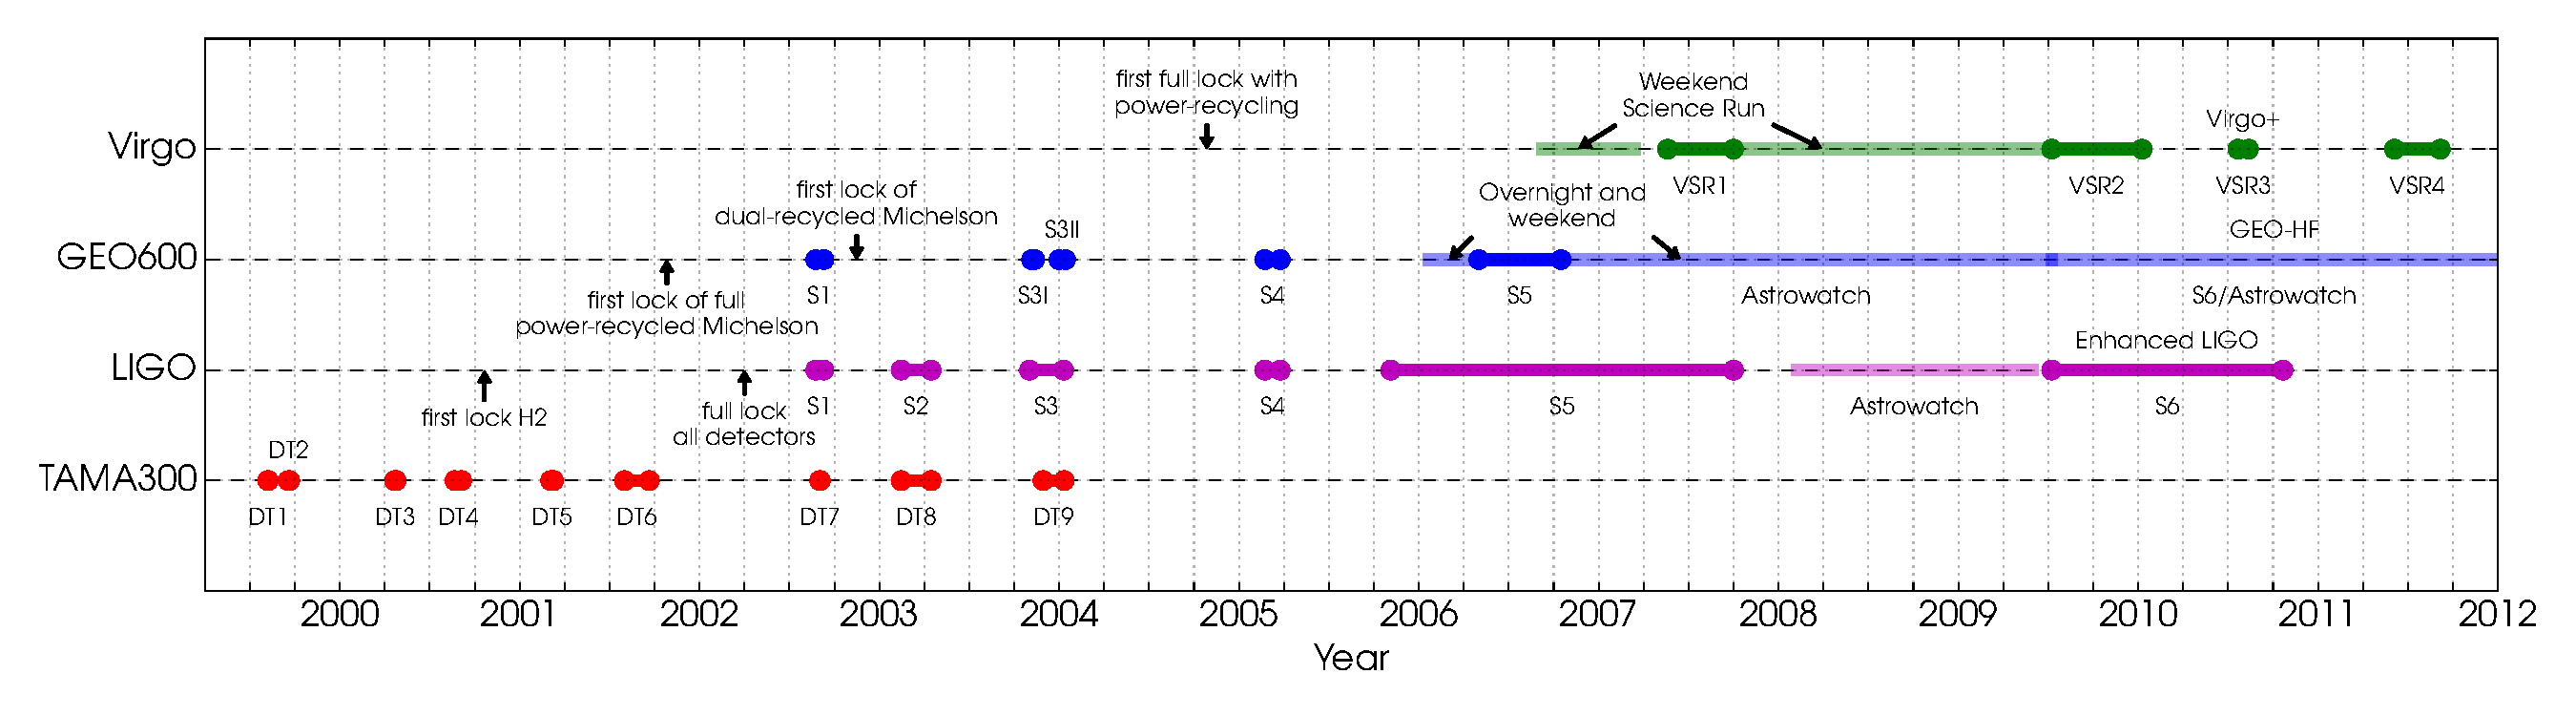
\includegraphics[width=1\columnwidth]{./figures/runtimes/runtimes}
\caption{ \protectA time-line of the science runs of the first generation
interferometric gravitational-wave detectors, from their first lock to
mid-2011.}
\end{center}
\end{figure}


\begin{figure}[]
\begin{center}
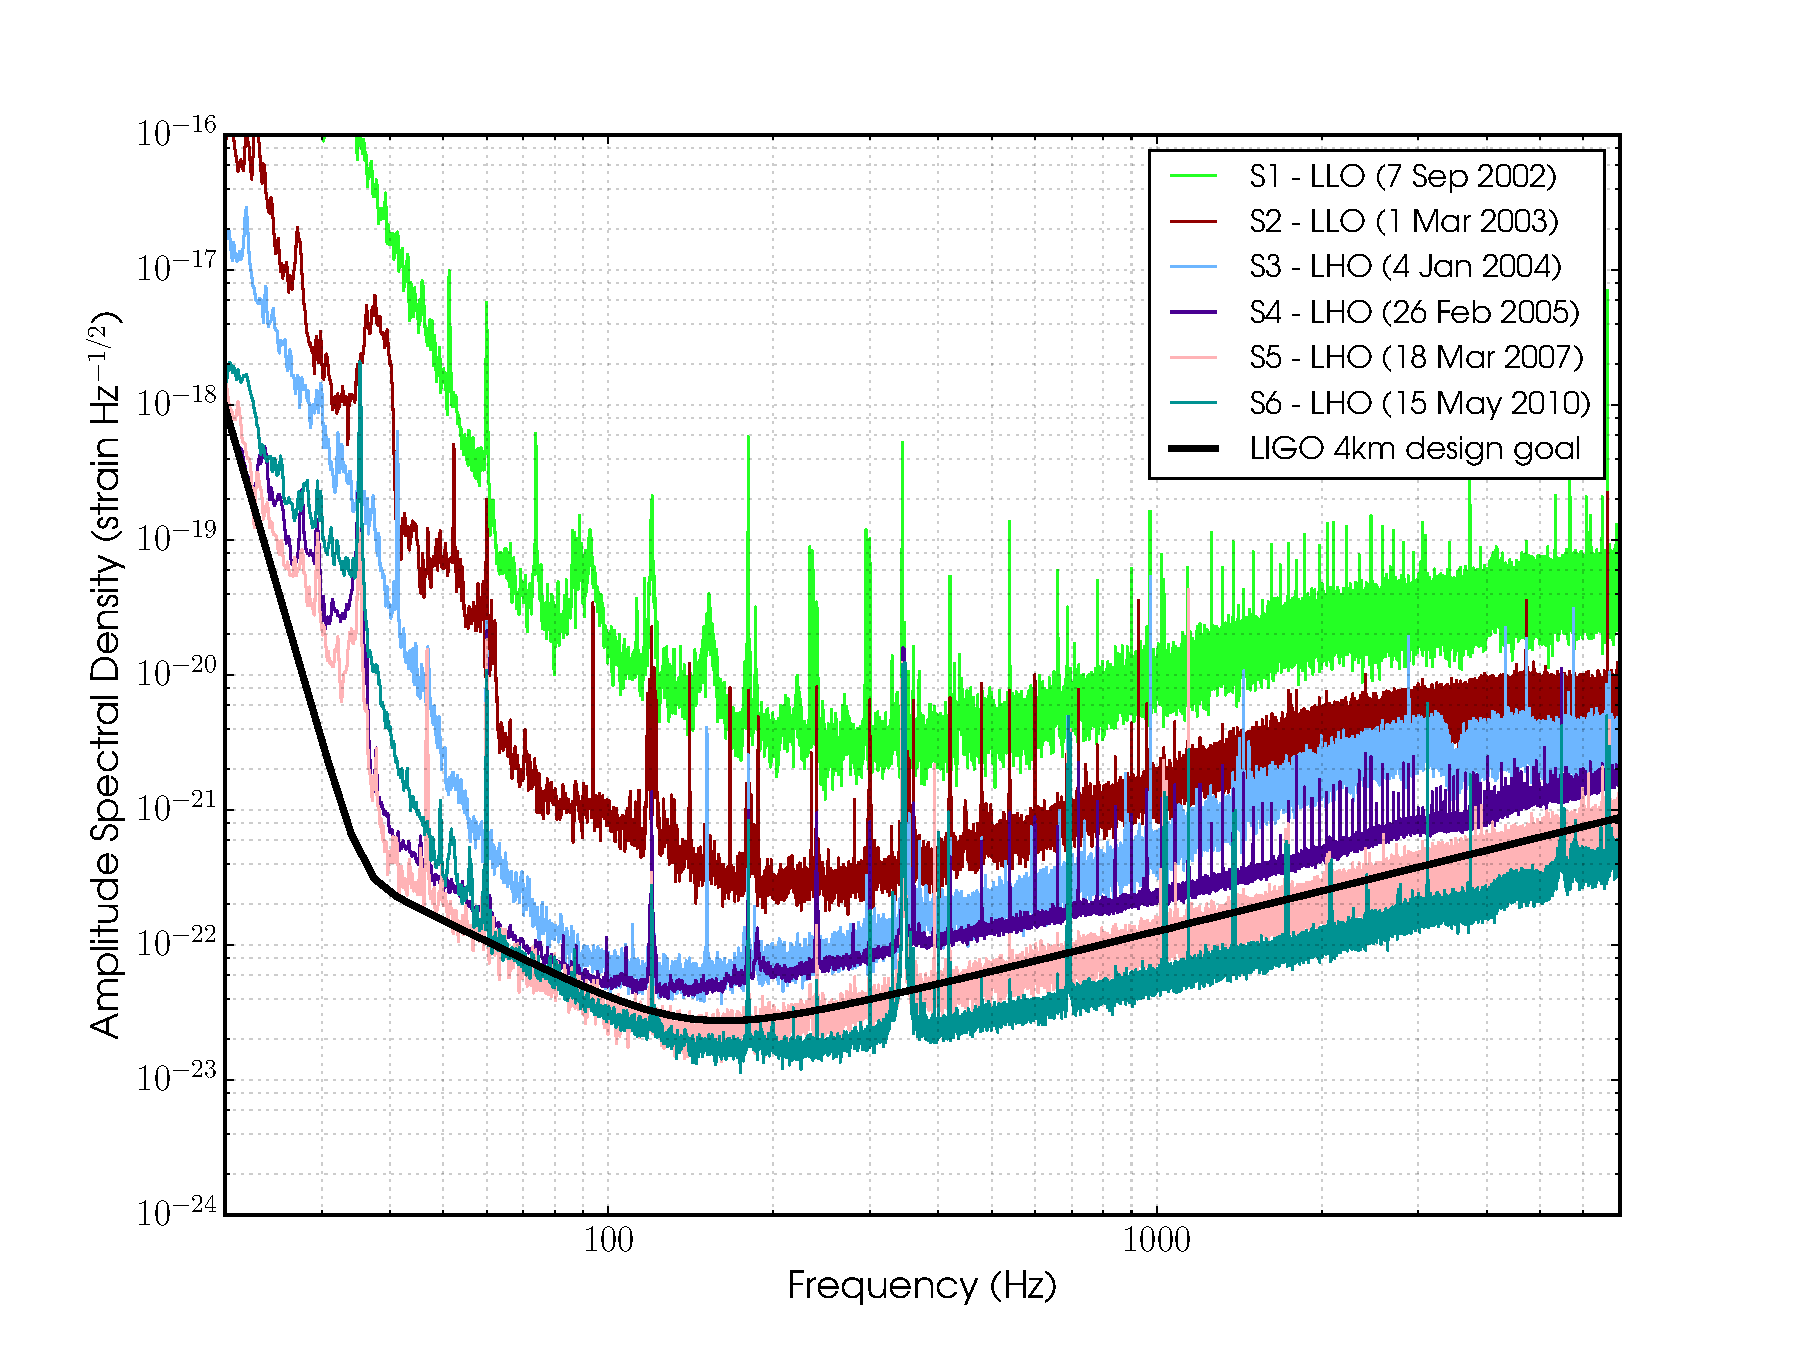
\includegraphics[width=1\columnwidth]{./figures/LIGOSrunASDs/LIGOSrunASDs}
\caption{ \protect\label{figure:LIGOstrains}
The best strain sensitivities from the LIGO science runs S1
through S6~\cite{LIGOcurves}. The S6 curve is preliminary and based on h(t) data
that has not been completely reviewed and may be subject to change. Also shown
is the LIGO 4~km design sensitivity.}
\end{center}
\end{figure}


\begin{figure}[]
\begin{center}
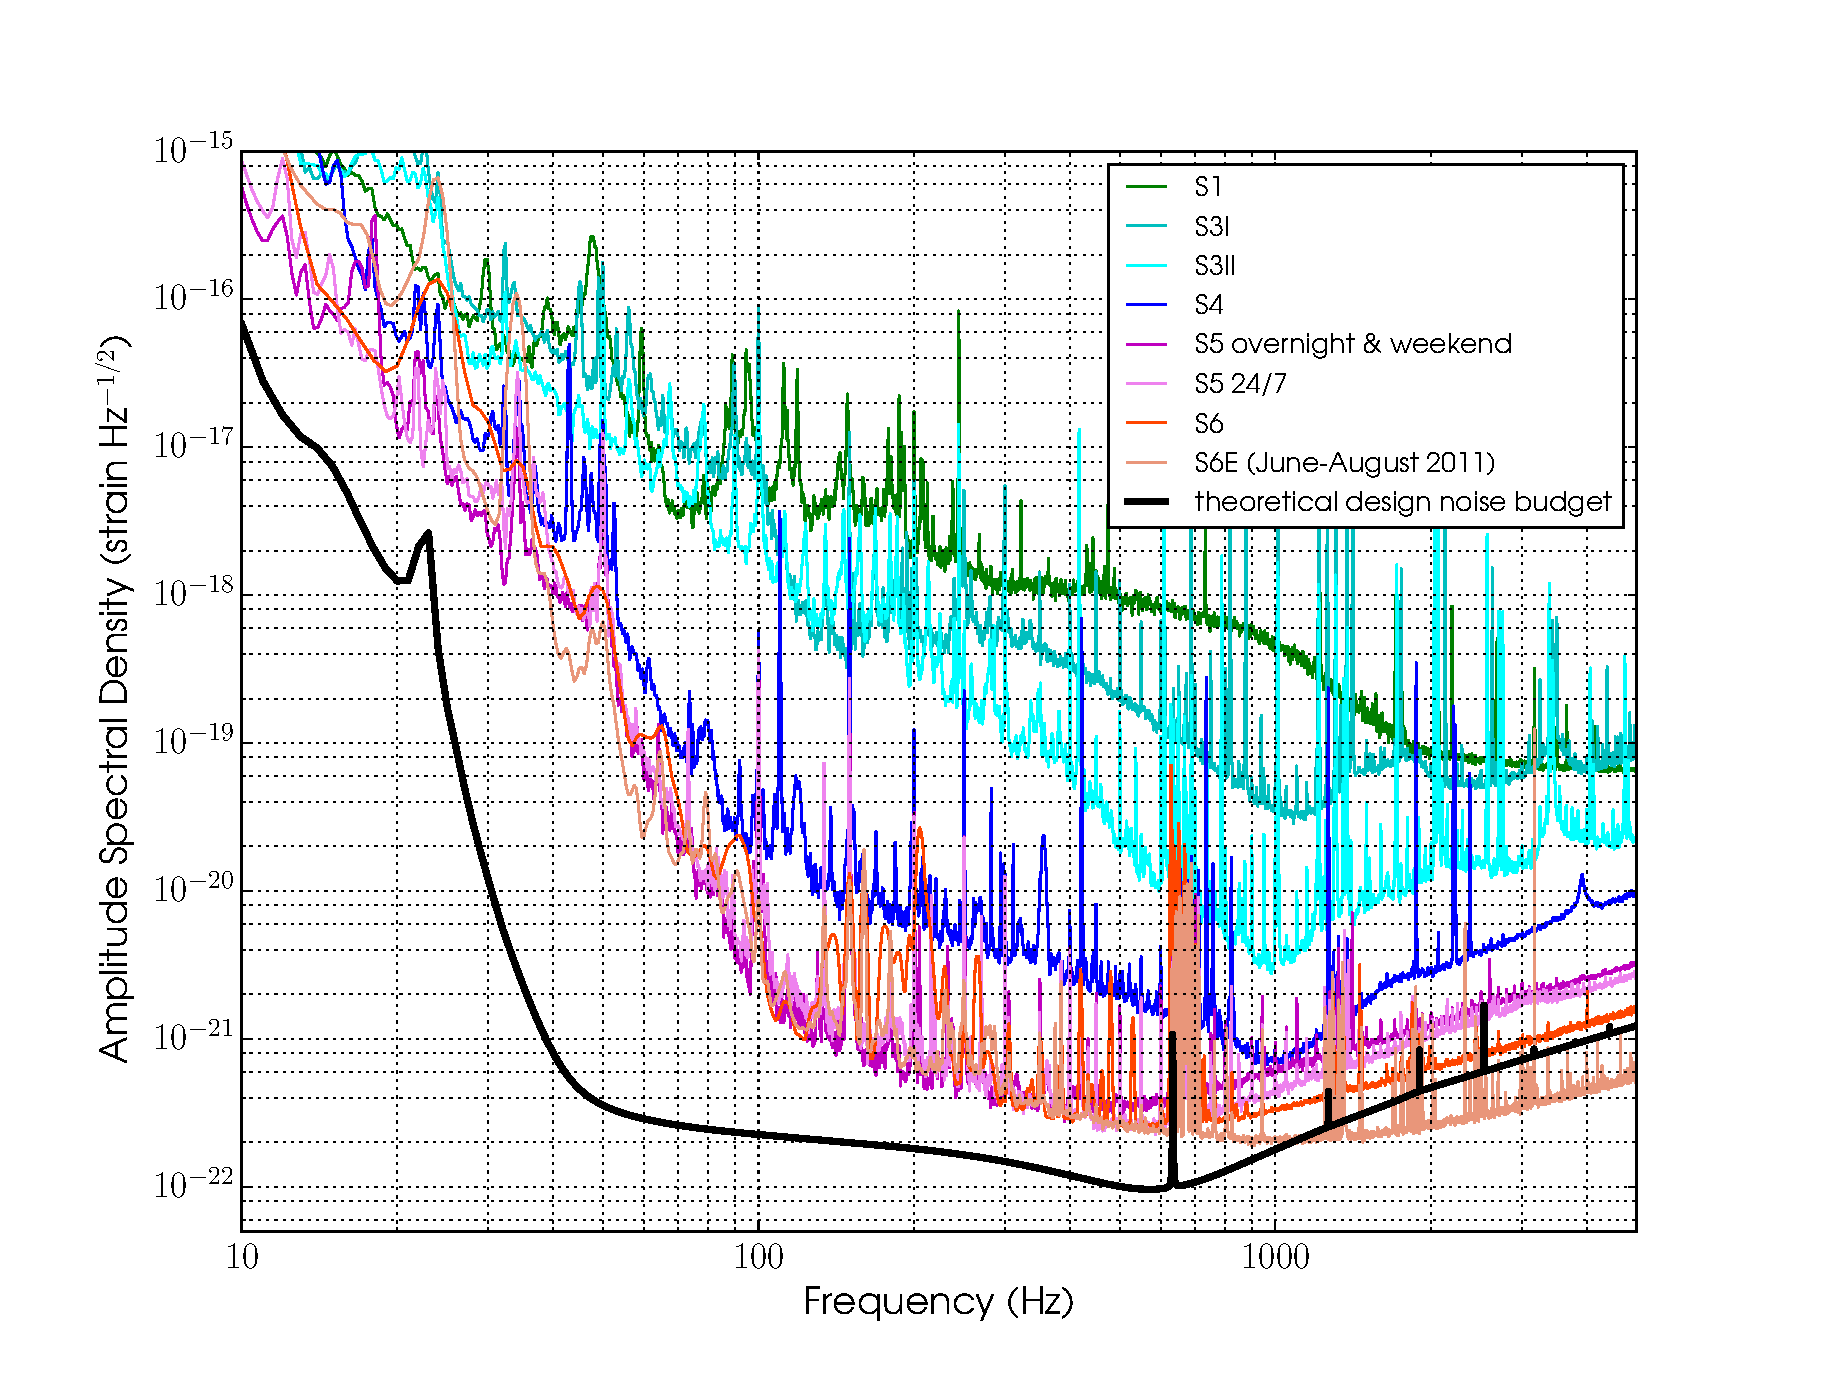
\includegraphics[width=1\columnwidth]{./figures/GEOSrunASDs/GEOSrunASDs}
\caption{ \protect\label{figure:GEOstrains}
The typical strain sensitivities from the GEO600 science runs S1
through S5~\cite{GEOcurves}. Also shown is the theoretical noise budget for the
detector when tuned to 550~Hz -- the operating position for the S5 run.
}
\end{center}
\end{figure}


\begin{figure}[]
\begin{center}
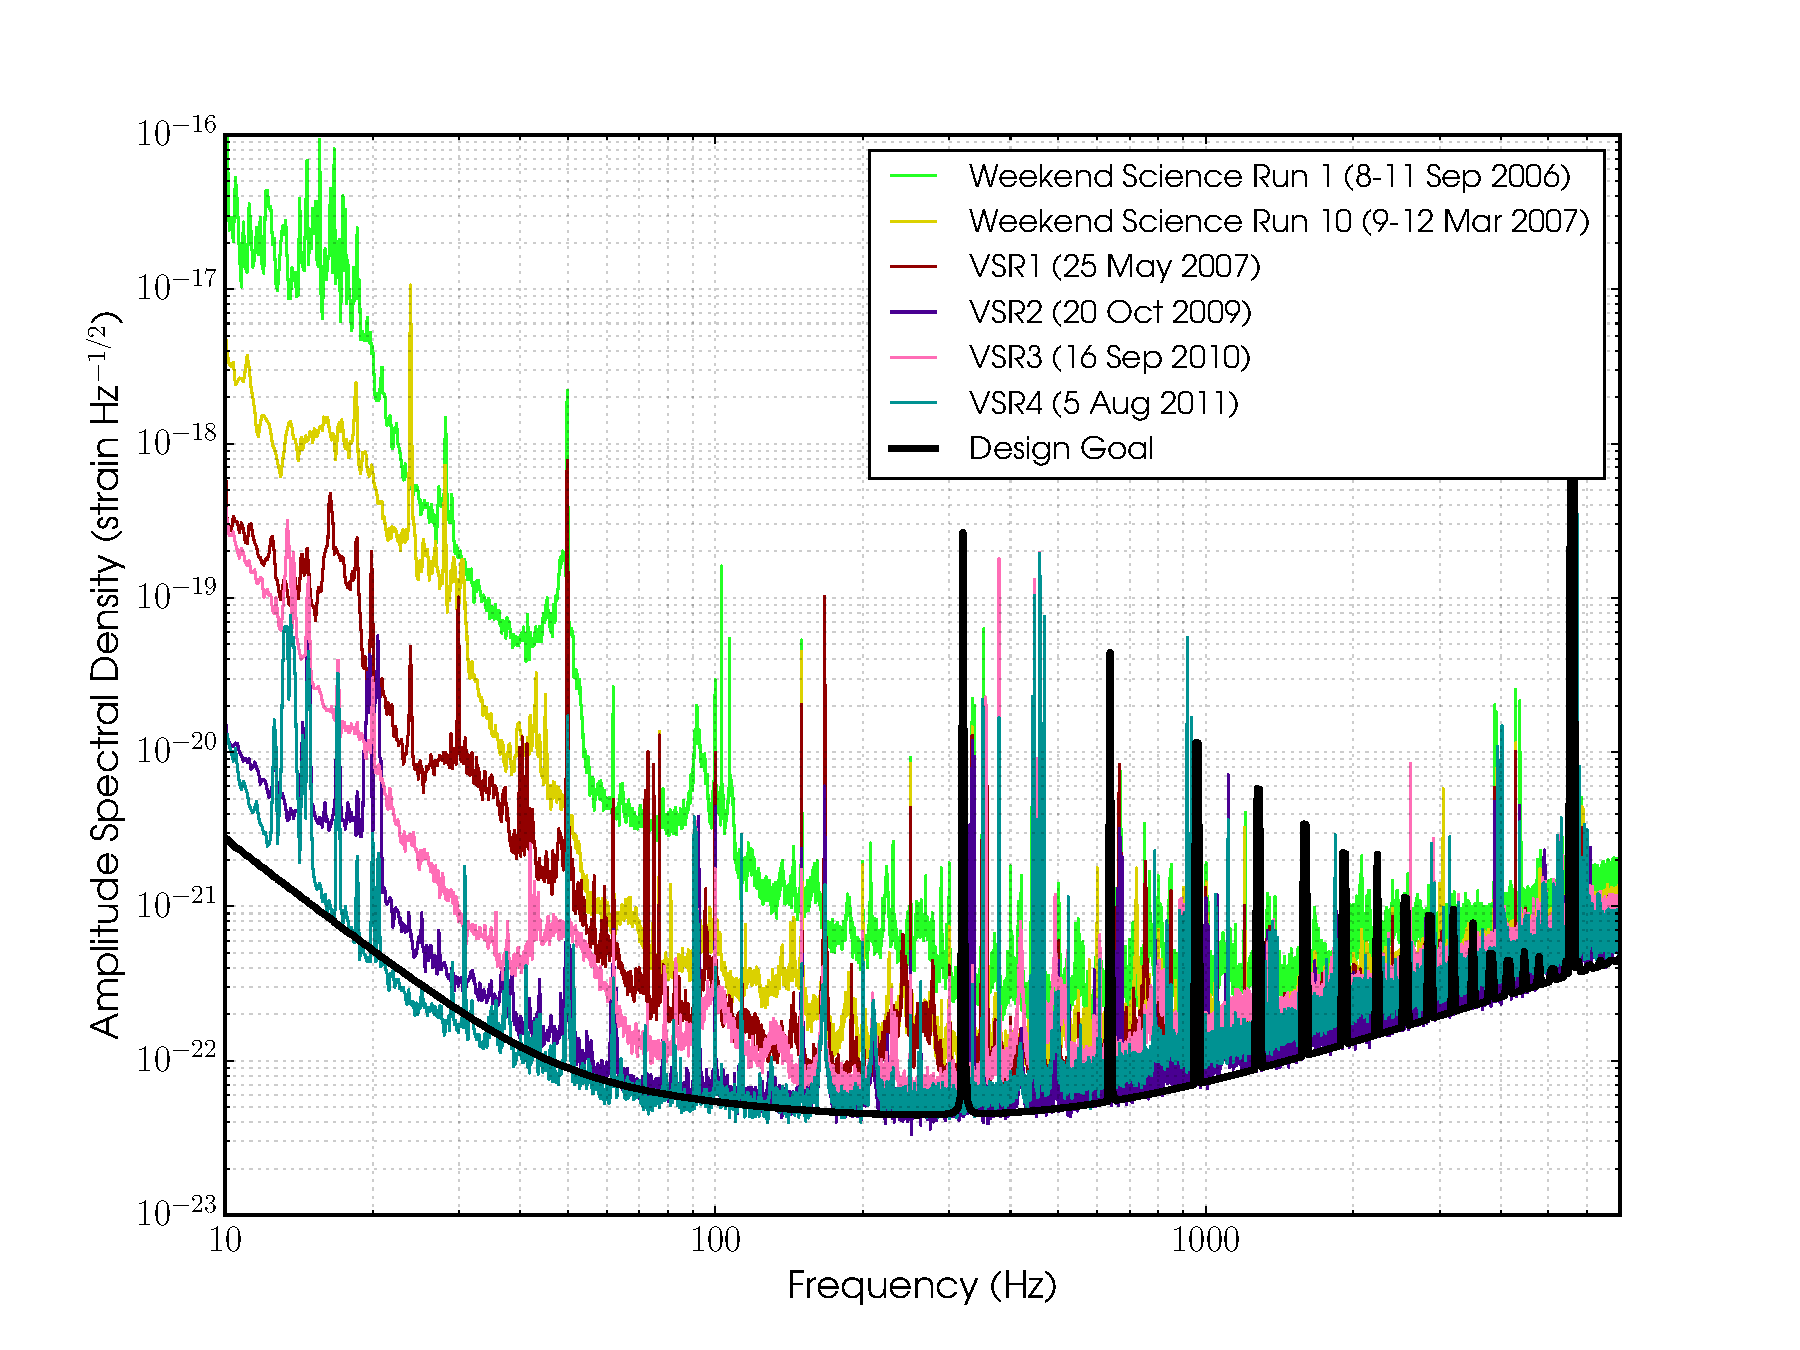
\includegraphics[width=1\columnwidth]{./figures/VirgoSrunASDs/VirgoSrunASDs}
\caption{ \protectThe best strain sensitivities from the Virgo weekend and full
time science runs WSR1, WSR10, VSR1 and VSR2~\cite{VIRGOcurves, VSR2paper}.}
\end{center}
\end{figure}


\begin{figure}[]
\begin{center}
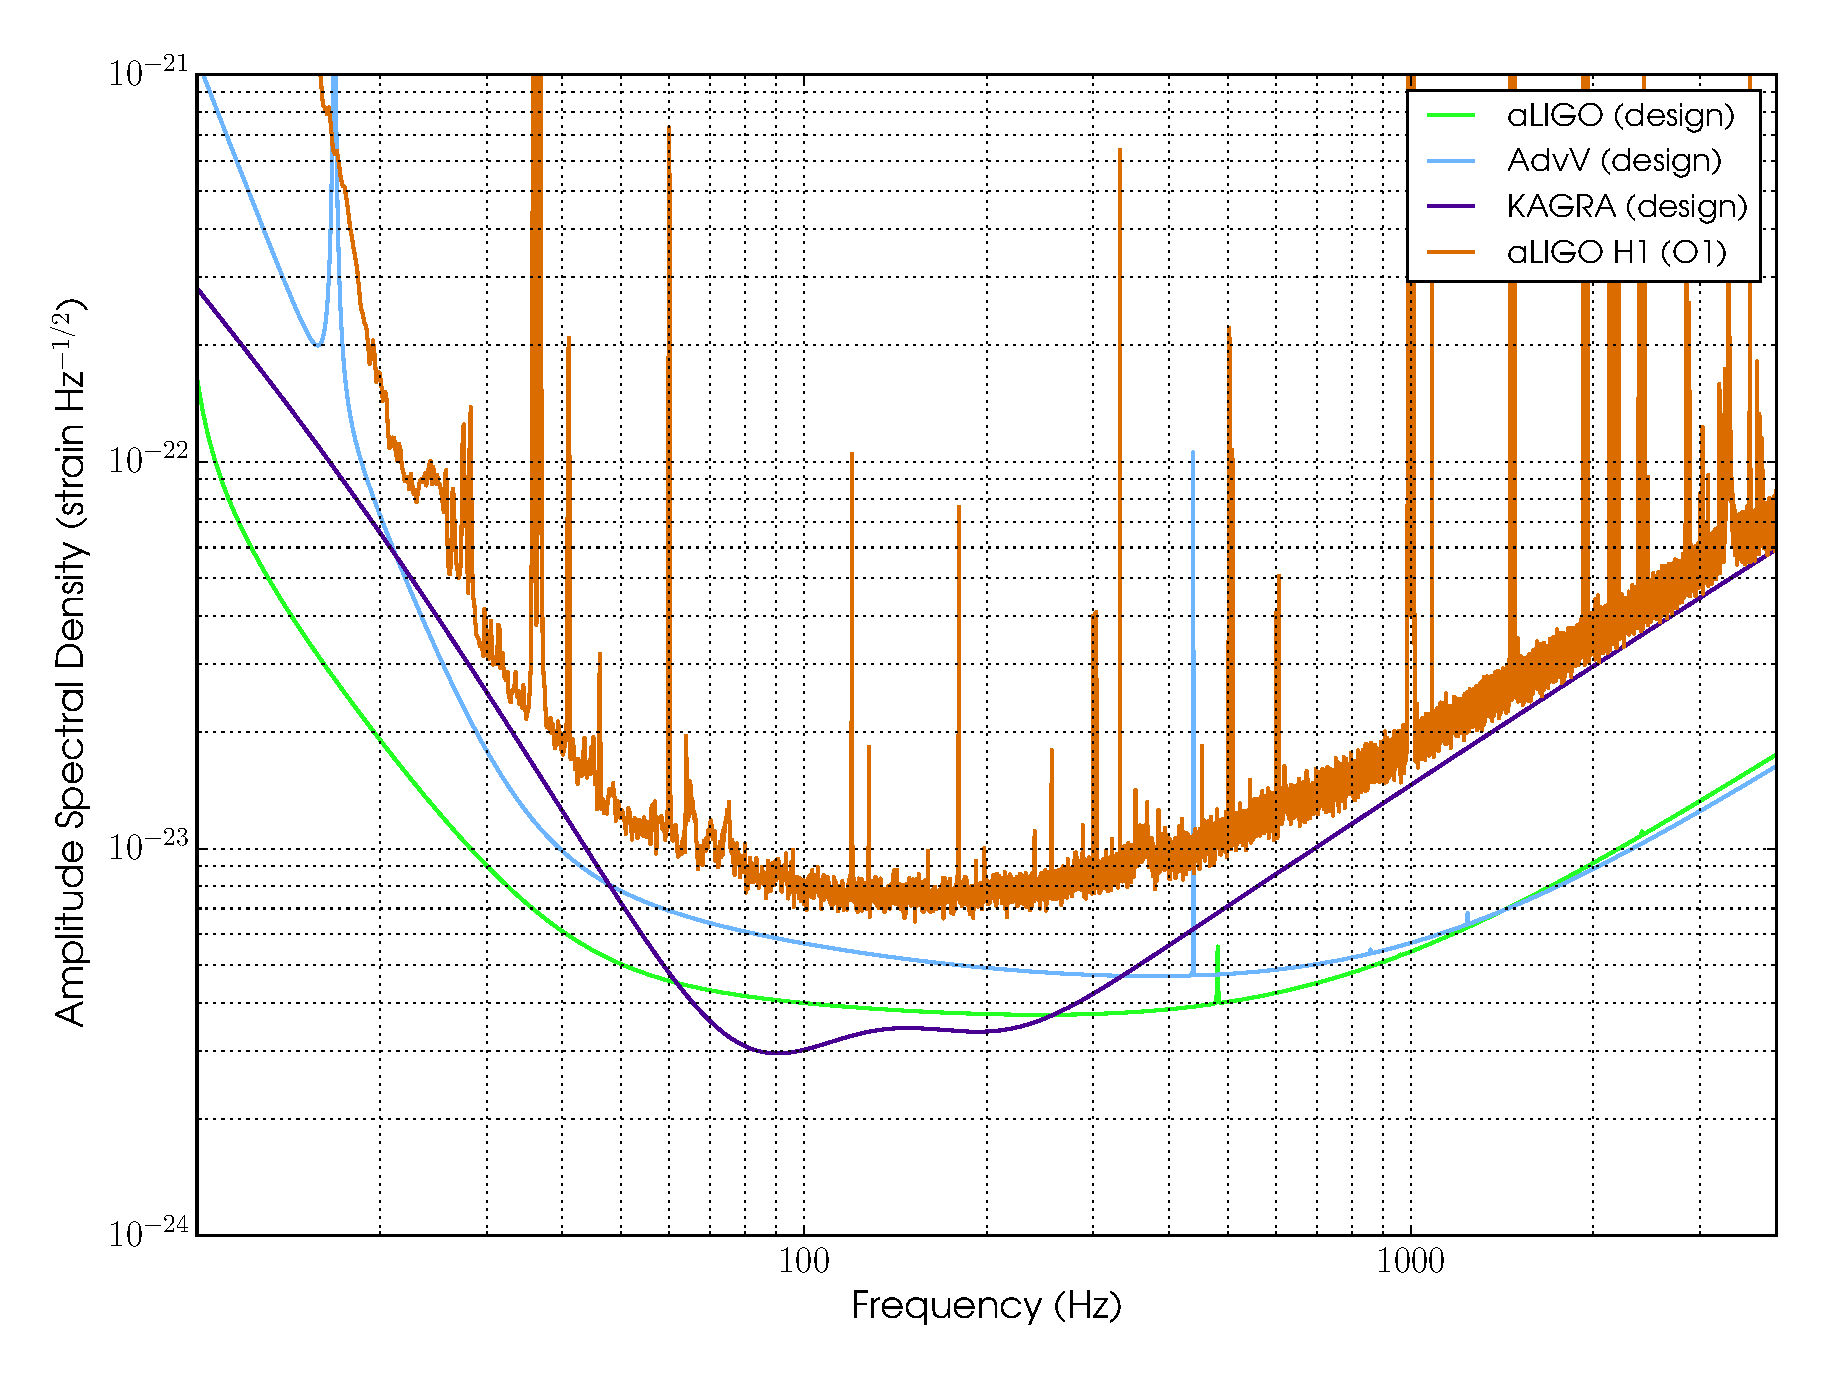
\includegraphics[width=1\columnwidth]{./figures/advcurves/advcurves}
\caption{ \protect\label{fig:advcurves}
Design sensitivity curves for the Advanced LIGO, Advanced Virgo
and LCGT second-generation detectors. The Advanced LIGO curve comes from
\cite{Harry:2010}, the Advanced Virgo curve comes
from~\cite{AdvVirgoweb}, and the LCGT curve comes
from~\cite{Arai:2009}. These curves are based on specific
configurations of the detectors and are therefore subject to change.
}
\end{center}
\end{figure}


\begin{figure}[]
\begin{center}
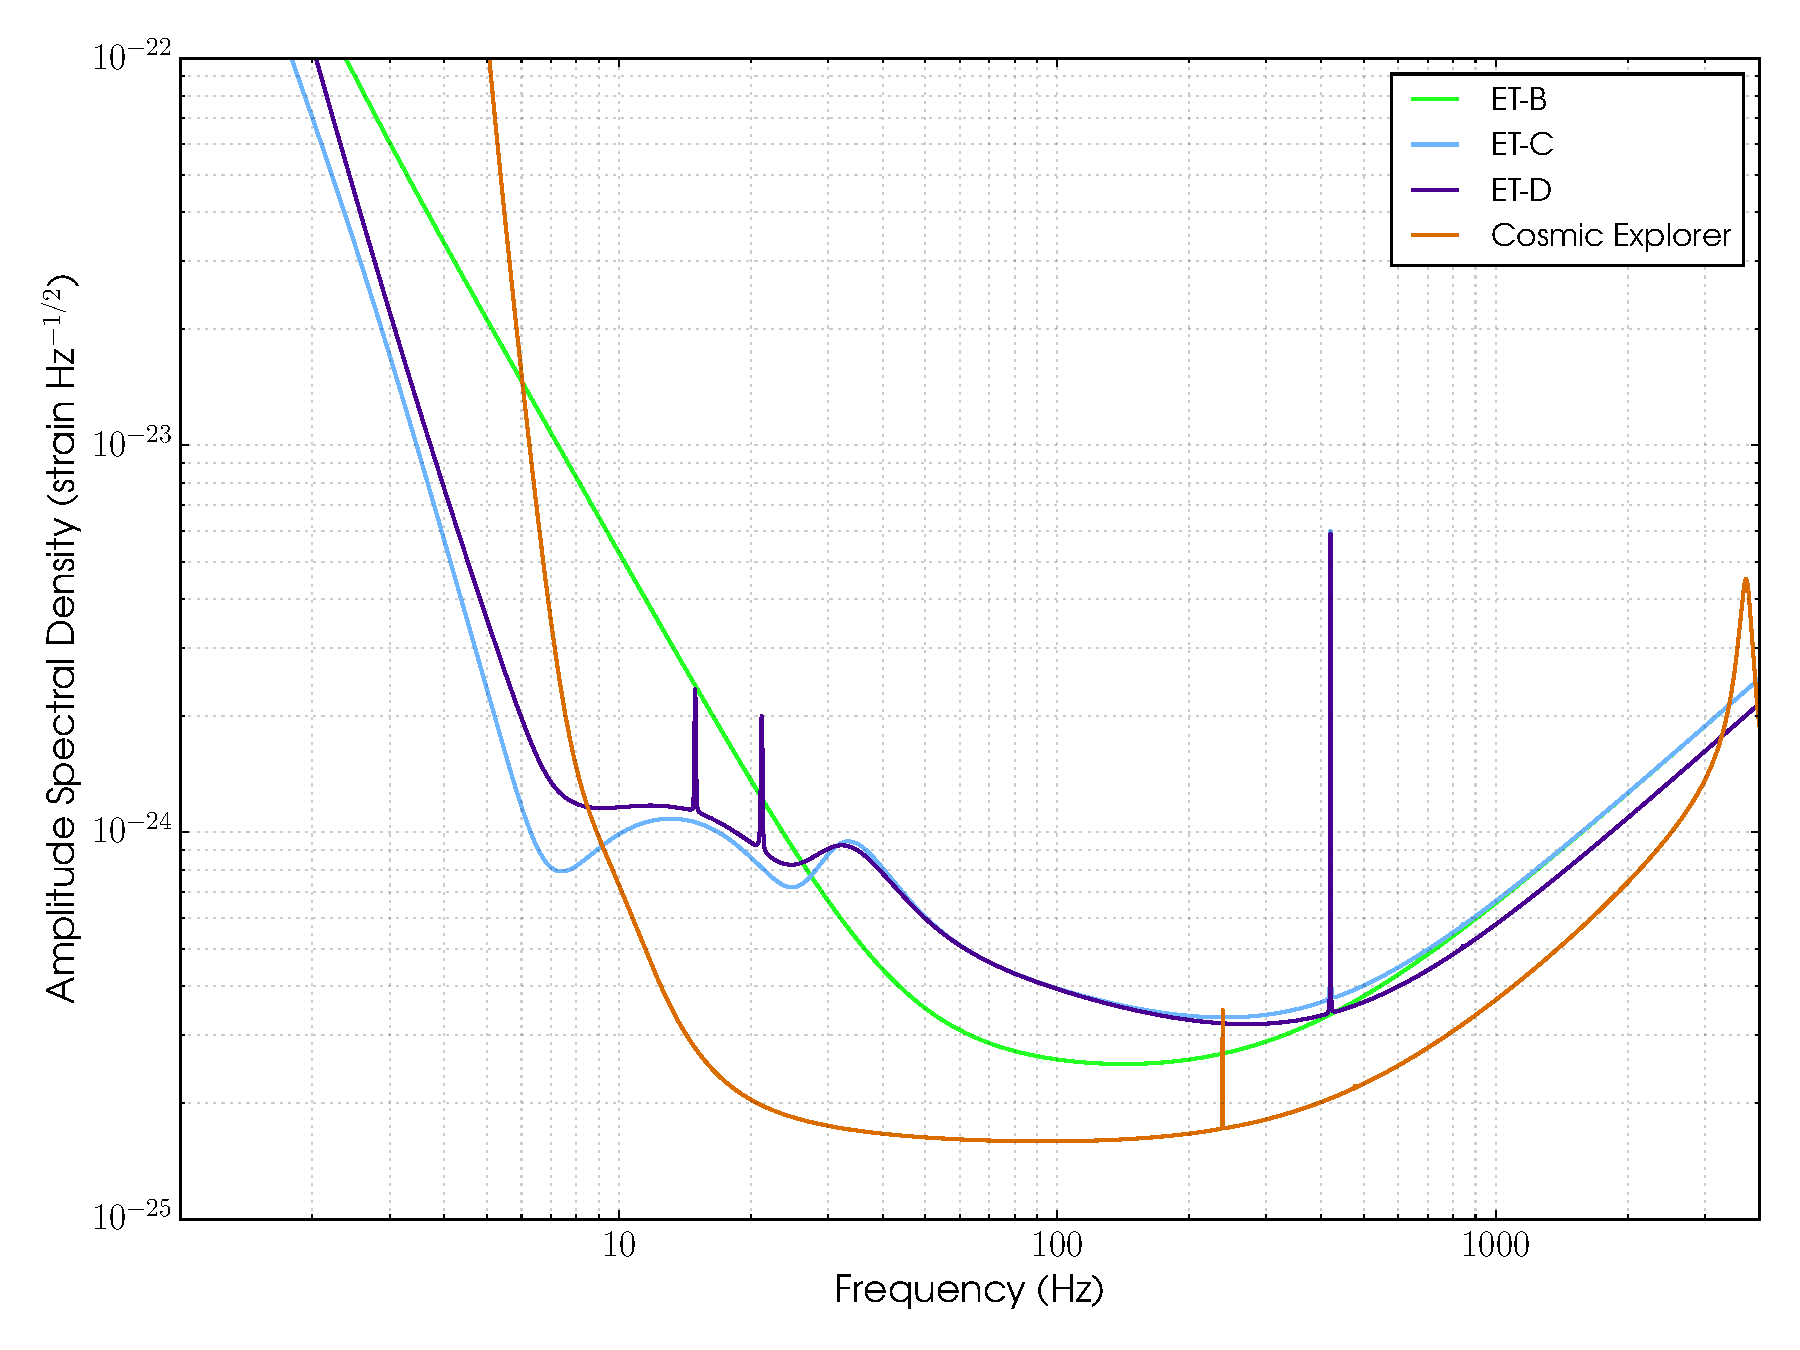
\includegraphics[width=1\columnwidth]{./figures/etcurve/etcurve}
\caption{ \protectPotential sensitivities of the Einstein Telescope for 3 different
design concepts: ET-B~\cite{Hild:2008}, ET-C~\cite{Hild:2010b} and ET-D
\cite{Hild:2010}. The curves are available from~\cite{etcurves}}
\end{center}
\end{figure}

\input{"./Section7"}

\begin{figure}[]
\begin{center}
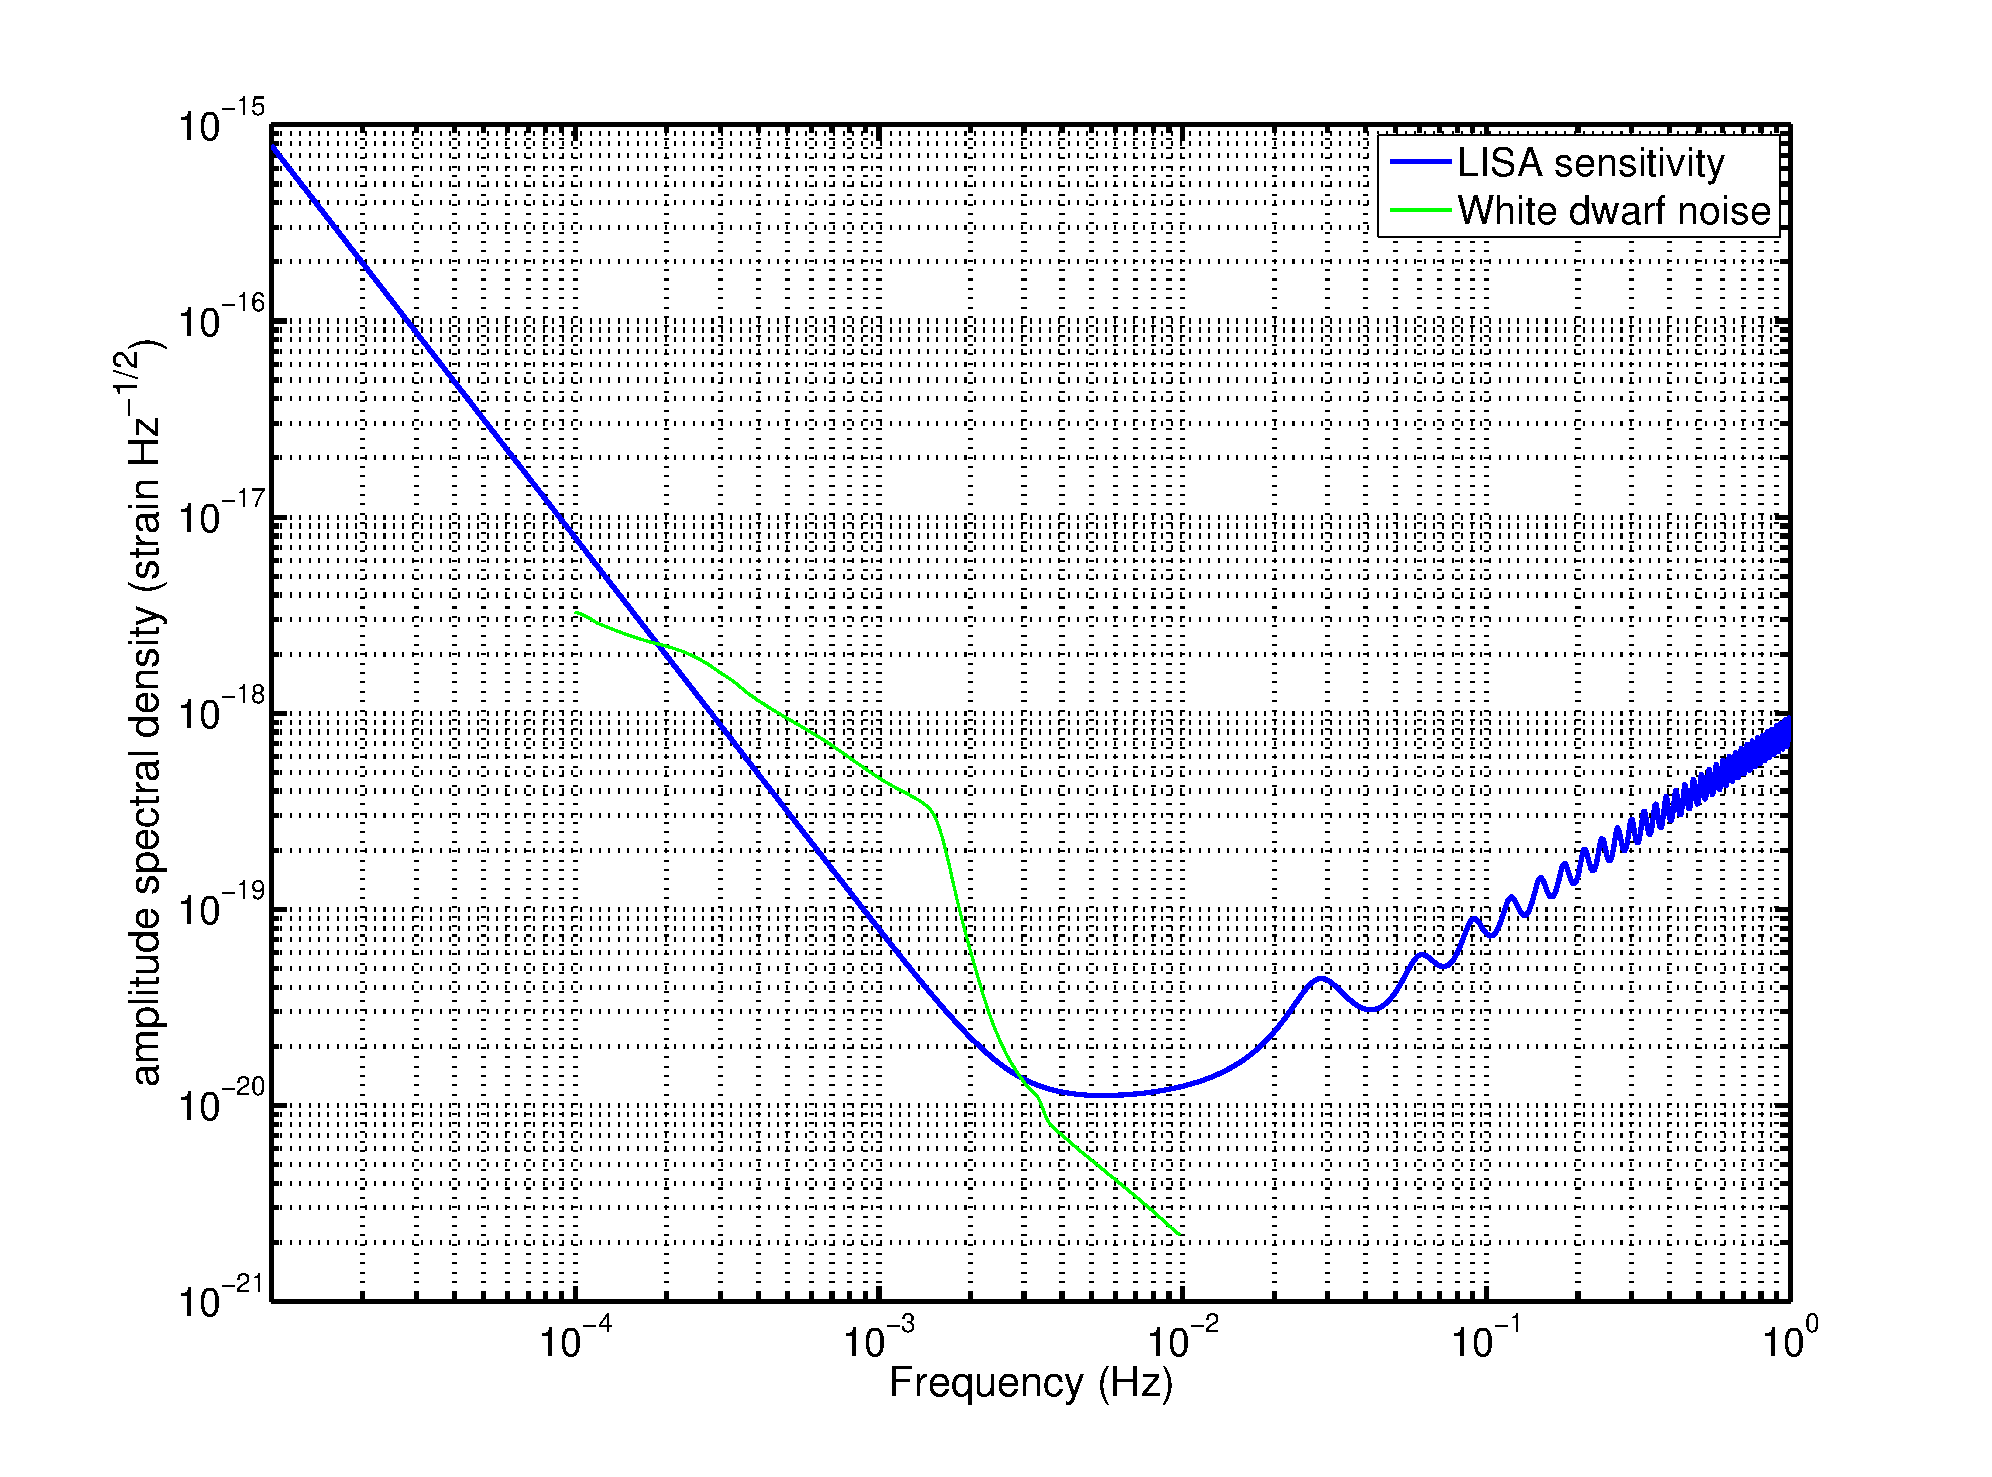
\includegraphics[width=1\columnwidth]{./figures/lisacurve/lisacurve}
\caption{ \protectA design sensitivity amplitude spectral density curve for LISA
created using the standard parameters in the online generator
at~\cite{lisasens}. The curve assumes equal length arms, sensitivity
averaged over the whole sky and all polarisations, and an SNR of
1. Also included is a curve showing the expected background noise from
galactic white-dwarf--binary systems, which will dominate over the
instrumental noise in the range from $\approx$~0.1\,--\,1~mHz.}
\end{center}
\end{figure}


\begin{figure}[]
\begin{center}
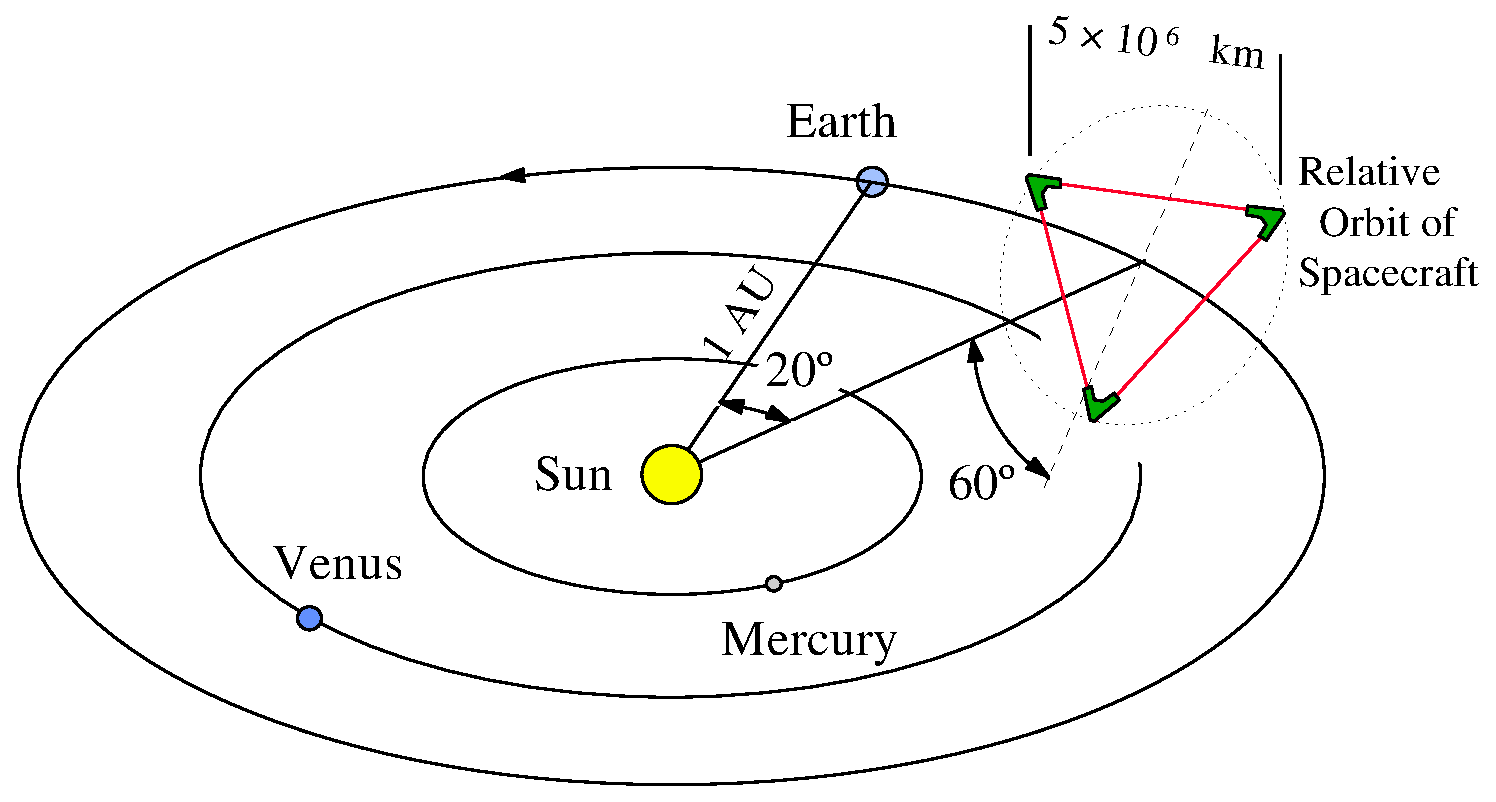
\includegraphics[width=1\columnwidth]{./figures/fig8/fig8}
\caption{ \protect\label{figure:LISA}
The proposed LISA detector.
}
\end{center}
\end{figure}

\input{"./Section8"}
\input{"./acknowledgements"}

\bibliography{./bibliography/biblio}{}

\end{document}
